\section{Inverse Kinematics}
\emph{Inverse Kinematics} aims at finding joint parameters that achieve a desired end-effector pose. This is a more complex problem than forward kinematics, as it is not always possible to find a solution, and when it is, there may be multiple solutions.
\begin{figure}[H]
    \centering
    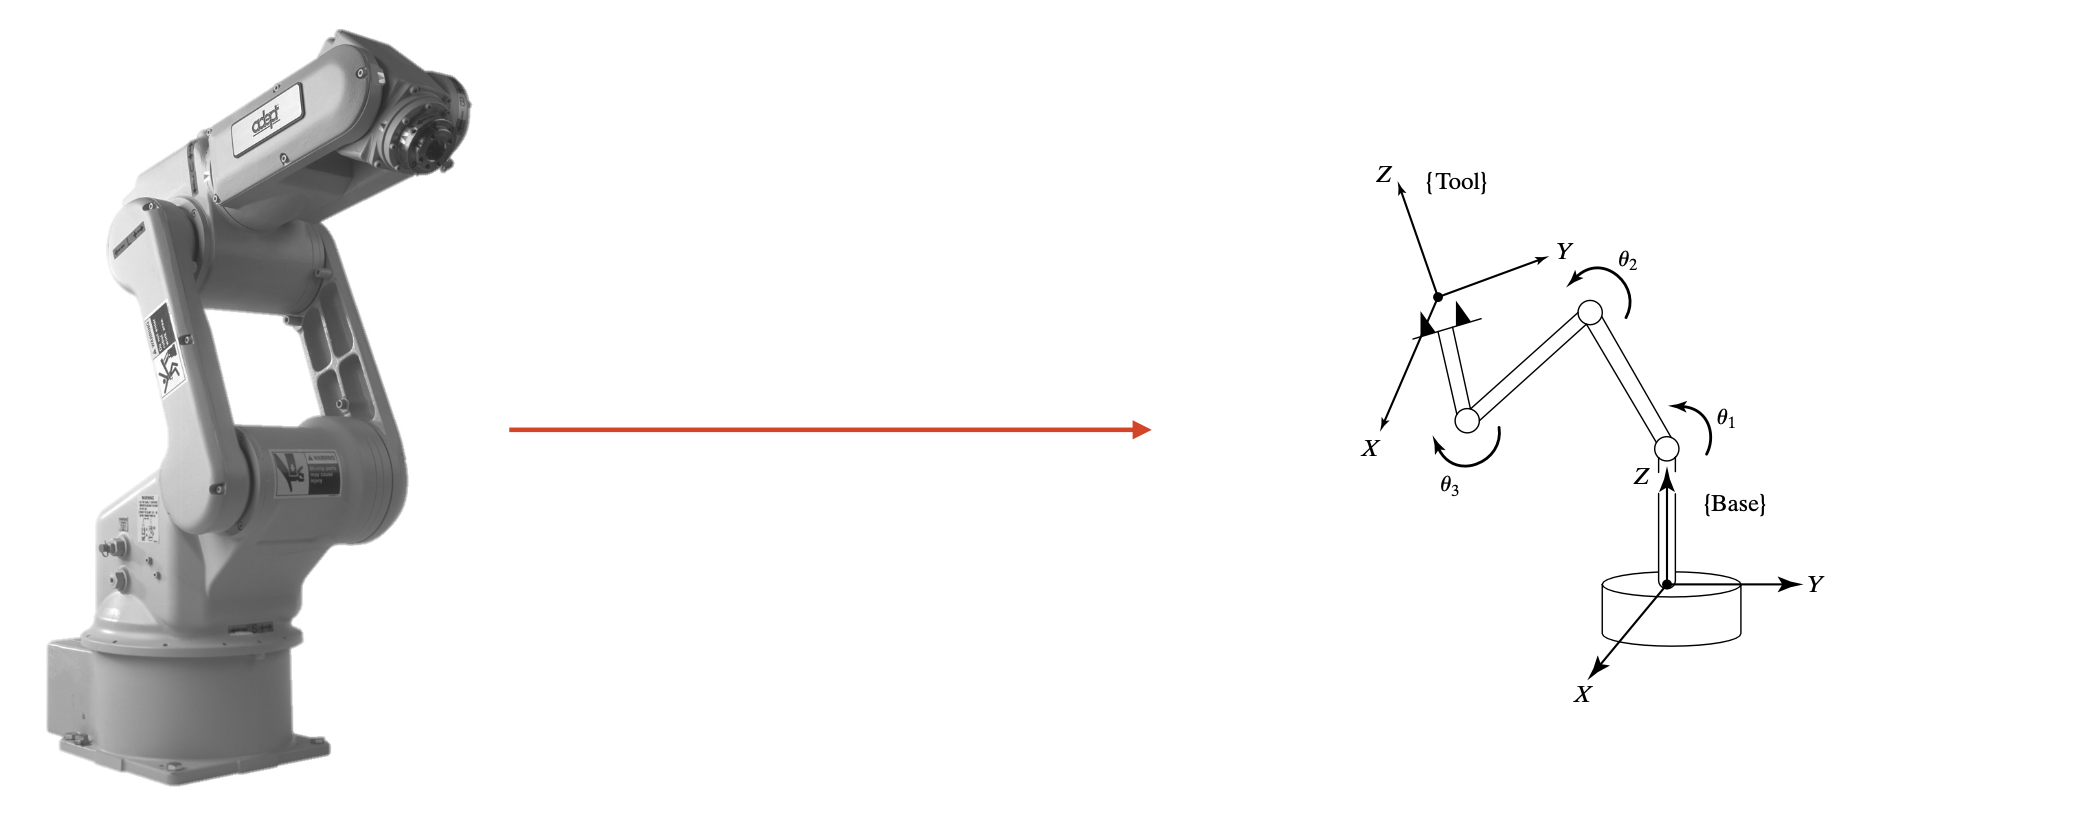
\includegraphics[width=0.8\textwidth]{inverse-kinematics/inverse-kinematics.png}
\end{figure}

\subsection{Optimization problem and resolution}
Given a target position $M^*$ for the end-effector, we aim at solving the following distance minimization problem:
\begin{equation*}
    \min_{q\in Q} d(\prescript{0}{}{K_n(q)}, M^*)
\end{equation*}
Using the logarithm distance, we can rewrite the problem as:
\begin{equation}
    \min_{q\in Q} \norm{\log(\prescript{0}{}{K_n(q)}^{-1}M^*)}
\end{equation}
We can cast this initial problem $\min_{q\in Q} \norm{\log(\prescript{0}{}{K_n(q)}^{-1}M^*)}$ as a more general optimization problem:
\begin{equation*}
    \min_{x\in\R^n}\frac{1}{2}\norm{f(x)}_2^2
\end{equation*}
We aim at iteratively solving this optimization problem. A first-order linear approximation of $f$ around $x$ is given by:
\begin{equation*}
    f(x+p)=f(x)+\underbrace{\partfrac{f}{x}(x)}_{J(x)}p
\end{equation*}
Hence:
\begin{equation*}
    \min_{p\in\R^n}\frac{1}{2}\norm{f(x_0+p)}_2^2 = \min_{p\in\R^n}\frac{1}{2}\norm{f(x)+J(x)p}_2^2
\end{equation*}
We can now solve the optimization problem by setting the gradient of the objective function to zero:
\begin{equation*}
    \begin{aligned}
        &\nabla_p\left(\frac{1}{2}\norm{f(x)+J(x)p^*}_2^2\right)=0\\
        \iff &J(x)^\tp (f(x)+J(x)p^*) = 0\\
        \iff &p^* = -(J(x)^\tp J(x))^{-1}J(x) f(x)\\
        \iff &p^* = -J(x)^+ f(x)
    \end{aligned}
\end{equation*}
where $J(x)^+$ is the \emph{Moore-Penrose pseudoinverse} of $J(x)$. We can then iteratively update:
\begin{equation*}
    x_{k+1} = x_k + \alpha p_k
\end{equation*}
until we obtain $\norm{J(x)^\tp f(x)}\leq\epsilon^*$, where $\epsilon^*>0$ is a fixed precision we aim at achieving. This iterative method is known as the \emph{Newton-Raphson} method. If we work on a differential manifold, we can use instead:
\begin{equation*}
    q_{k+1}=q_l\oplus\alpha p_k
\end{equation*}

\subsection{Trajectory tracking}
We can extend the previous method to track a trajectory $M(t)$: we want to compute the joint speeds $\dot{q}$ that track the trajectory as closely as possible. Consider a continuous and differentiable time trajectory $M^*$:
\begin{equation*}
    \begin{aligned}
        M^*:[0, T]&\longrightarrow \SE(3)\\
        t&\longmapsto M^*(t)
    \end{aligned}
\end{equation*}
We are also given the corresponding spatial (linear and angular) velocity of the end-effector $v^*$:
\begin{equation*}
    \begin{aligned}
        v^*:[0, T]&\longrightarrow\se(3)\\
        t&\longmapsto v^*(t)
    \end{aligned}
\end{equation*}

At each instant $t$, the forward kinematics of the robot give us the current end-effector pose $M(t)$ and the corresponding Jacobian $J(t)$:
\begin{equation*}
    M(q(t)) = \bigtimes_{i=0}^n K_i(q_i(t)) \in\SE(3)
    \quad\text{and}\quad
    v(t) = J(q(t))\dot{q}(t)\in\se(3)
\end{equation*}
Using the angular speed of the joints $\dot{q}(t)$, we can control the position $q(t)$ of the joints. Our goal is to minimize the gap between the position and speed of the end-effector $(M(q(t)), v(q(t), \dot{q}(t)))$ and the desired trajectory $(M^*(t), v^*(t))$.

The error can be computed using the following cost function:
\begin{equation*}
    e(t, q(t)) = M(q(t)) \ominus M^*(t) = \log_{\SE(3)}\left(M^*(t)^{-1}M(q(t))\right)
\end{equation*}
The error in velocity space is given by:
\begin{equation*}
    \dot{e}(t, q(t), \dot{q}(t)) = v(q(t), \dot{q}(t)) - v^*(t) = J(q(t))\dot{q}(t) - v^*(t)
\end{equation*}
We define the error correction profile as:
\begin{equation*}
    \dot{e}(t, q(t), \dot{q}(t)) = -\lambda e(t, q(t))
\end{equation*}
for some $\lambda>0$. 

We would like to have $\dot{e}+\lambda e=0$ to respect the error correction profile. Therefore, we want to solve the following optimization problem:
\begin{equation}
    \min_{\dot{q}(t)} \frac{1}{2}\norm{\dot{e}+\lambda e}_2^2
\end{equation}
By substituting the expressions of $e$ and $\dot{e}$, we obtain:
\begin{equation*}
    \min_{\dot{q}(t)} \frac{1}{2}\norm{
        \underbrace{J(q(t))}_{A}\underbrace{\dot{q}(t)}_{x} - \underbrace{v^*(t) + \lambda\left(M(q)\ominus M^*\right)}_{b}
    }_2^2
\end{equation*}
This is a linear least squares problem, i.e. of the form:
\begin{equation*}
    \min_{x\in\R^n}\frac{1}{2}\norm{Ax-b}_2^2
\end{equation*}
with $A=J(q(t))$ and $b=v^*(t)+\lambda\left(M(q)\ominus M^*\right)$. The solution is given by:
\begin{equation*}
    x^* = A^+b = (A^\tp A)^{-1}A^\tp b
\end{equation*}
We can then update the joint speeds $\dot{q}(t)$ using the computed values $x^*$.

\subsection{Exploiting the redundancy of solutions}
In the case of redundant robots, there are multiple solutions to the inverse kinematics problem. We can exploit this redundancy to optimize a given criterion. For instance, we can minimize the energy consumption of the robot by minimizing the norm of the joint speeds.

More generally, we can consider two tasks to be achieved simultaneously, one being strictly prioritized over the other:
\begin{equation*}
    (A_1, b_1) \gg (A_2, b_2)
\end{equation*}

\subsubsection{Relaxed approach}
A first approach is to assign each task a coefficient $\alpha_i>0$, and to choose the cost function to be the sum of the weighted tasks. Given $\alpha_1\gg\alpha_2>0$, we might want to minimize:
\begin{equation*}
    \min_x\alpha_1\norm{A_1x+b_1}_2^2 + \alpha_2\norm{A_2x+b_2}_2^2
\end{equation*}
However, this approach does not guarantee that the first task will be strictly prioritized over the second one. Imagine that the first task is for our robot to stay in a safe position, while the second task is to reach a target position. To ensure that the robot stays in a safe position, we need to strictly prioritize the first task, resulting in a much higher $\alpha_1$ than $\alpha_2$. This would lead to a numerically unstable problem, and the robot would likely not reach the target position.

\subsubsection{Strict approach}
A more stable approach consists in solving a constrained optimization problem:
\begin{equation*}
    \min_x\norm{A_2x+b_2}_2^2 \quad\text{s.t. } A_1x=b
\end{equation*}
This guarantees that the first task is strictly prioritized over the second one, and does not require coefficients. To do so, we can compute the projection of the second task onto the null space of the first task. For any problem of the form:
\begin{equation*}
    \min_x\norm{Ax-b}_2^2
\end{equation*}
a solution is given by $x^*=A^+b$. If $A$ is not invertible (which is the case when the system is underdetermined), the solutions are given by:
\begin{equation*}
    x^* = A^+b + \underbrace{(I-A^+A)}_{P_{\ker(A)}}y
\end{equation*}
for some $y\in\R^n$. The general idea of minimizing the second task while respecting the first one is to choose the value of $y$ that minimizes the norm of the second task. This is equivalent to projecting the second task onto the null space of the first task.

Given two tasks $(A_1, b_1)\gg(A_2, b_2)$, we want to choose $y$ such that:
\begin{alignat*}{2}
    &&A_2(A_1^+b_1 + (I-A_1^+A_1)y) &= b_2\\
    \iff &&\underbrace{A_2(I-A_1^+A_1)}_{\tilde{A}_2}y &= \underbrace{b_2 - A_2A_1^+b_1}_{\tilde{b}_2}\\
    \iff &&y &= \tilde{A}_2^+\tilde{b}_2
\end{alignat*}
Hence, we obtain the solution to the constrained optimization problem:
\begin{equation*}
    x^* = A_1^+b_1 + (I-A_1^+A_1)\tilde{A}_2^+\tilde{b}_2
\end{equation*}